\documentclass[11pt]{article}
\usepackage[margin=1in]{geometry}
\usepackage{fontspec}
\usepackage{amsmath,amssymb}
\usepackage{booktabs,tabularx,multirow}
\usepackage[numbers,sort&compress]{natbib}
\usepackage{xcolor}
\usepackage{pgfplots}
\pgfplotsset{compat=1.18}
\usetikzlibrary{positioning,fit,arrows.meta,backgrounds}
\usepackage{caption}
\usepackage{enumitem}
\usepackage[hidelinks]{hyperref}
\usepackage{url}
% generated by scripts/build_data.py -- do not edit
\newcommand{\CSeightAllFour}{6}
\newcommand{\CSeightBvsTS}{6}
\newcommand{\CSeightCalls}{3{,}200}
\newcommand{\CSeightDeightHit}{3}
\newcommand{\CSeightDup}{14}
\newcommand{\CSeightIAFour}{8}
\newcommand{\CSeightIAOne}{14}
\newcommand{\CSeightIAThree}{14}
\newcommand{\CSeightIATwo}{10}
\newcommand{\CSeightKfour}{16.0}
\newcommand{\CSeightKone}{11.5}
\newcommand{\CSeightKthree}{15.5}
\newcommand{\CSeightKtwo}{14.3}
\newcommand{\CSeightOutM}{3.68}
\newcommand{\CSeightOverTW}{1.5}
\newcommand{\CSeightPvsTS}{0.0156}
\newcommand{\CSeightSum}{46}
\newcommand{\CSeightTMhi}{14}
\newcommand{\CSeightTMlo}{12}
\newcommand{\CSeightTWonlyHit}{5}
\newcommand{\CSeightToolCalls}{3{,}175}
\newcommand{\CSeightUnion}{16}
\newcommand{\CSeightVsTWp}{1.0}
\newcommand{\CSfiveKeichOne}{0.1081949}
\newcommand{\CSfiveN}{10}
\newcommand{\CSfiveOneMatch}{4}
\newcommand{\CSfiveOneValid}{5}
\newcommand{\CSfiveOutRatioAll}{4.7}
\newcommand{\CSfiveSOneCalls}{341}
\newcommand{\CSfiveSOneOutM}{0.24}
\newcommand{\CSfiveSThreeCalls}{1{,}401}
\newcommand{\CSfiveSThreeOutM}{1.25}
\newcommand{\CSfiveSTwoCalls}{1{,}257}
\newcommand{\CSfiveSTwoOutM}{1.12}
\newcommand{\CSfiveThreeMatch}{3}
\newcommand{\CSfiveThreeValid}{10}
\newcommand{\CSfiveTwoMatch}{4}
\newcommand{\CSfiveTwoValid}{10}
\newcommand{\CSfourN}{7}
\newcommand{\CSfourOutRatioAll}{4.1}
\newcommand{\CSfourSOneCalls}{201}
\newcommand{\CSfourSOneMatch}{3}
\newcommand{\CSfourSOneOutM}{0.13}
\newcommand{\CSfourSOneValid}{7}
\newcommand{\CSfourSTwoCalls}{971}
\newcommand{\CSfourSTwoMatch}{5}
\newcommand{\CSfourSTwoOutM}{0.53}
\newcommand{\CSfourSTwoValid}{7}
\newcommand{\CSfourTimeOne}{99}
\newcommand{\CSfourTimeTwo}{33}
\newcommand{\CSnineB}{2}
\newcommand{\CSnineC}{0}
\newcommand{\CSnineLossTS}{45}
\newcommand{\CSnineLossTW}{15}
\newcommand{\CSnineOutRatio}{3.7}
\newcommand{\CSnineP}{0.25}
\newcommand{\CSnineTS}{11}
\newcommand{\CSnineTSCalls}{697}
\newcommand{\CSnineTSOutM}{0.65}
\newcommand{\CSnineTW}{13}
\newcommand{\CSnineTWCalls}{1{,}807}
\newcommand{\CSnineTWOutM}{2.45}
\newcommand{\CSnineTangoHi}{7.0}
\newcommand{\CSnineTangoLo}{-1.8}
\newcommand{\CSnineToolCalls}{2{,}368}
\newcommand{\CSsevenAugN}{34}
\newcommand{\CSsevenAugTS}{10}
\newcommand{\CSsevenAugTW}{13}
\newcommand{\CSsevenB}{6}
\newcommand{\CSsevenBoth}{10}
\newcommand{\CSsevenC}{0}
\newcommand{\CSsevenCallRatio}{3.9}
\newcommand{\CSsevenCondHi}{6.0}
\newcommand{\CSsevenCondLo}{0.5}
\newcommand{\CSsevenDiff}{6}
\newcommand{\CSsevenErdosN}{18}
\newcommand{\CSsevenExtraCallsPer}{250}
\newcommand{\CSsevenExtraOutPerK}{319}
\newcommand{\CSsevenFileB}{5}
\newcommand{\CSsevenFileC}{0}
\newcommand{\CSsevenFileP}{0.031}
\newcommand{\CSsevenFiles}{89}
\newcommand{\CSsevenFinalAfterMinTS}{283}
\newcommand{\CSsevenFinalAfterMinTW}{283}
\newcommand{\CSsevenFinalByMinTS}{343}
\newcommand{\CSsevenFinalByMinTW}{344}
\newcommand{\CSsevenLedgerFirstTS}{63}
\newcommand{\CSsevenLedgerFirstTW}{12}
\newcommand{\CSsevenMeanConc}{3.6}
\newcommand{\CSsevenMonthRows}{August 2026 & 34 & 10 & 13 \\ September 2026 & 45 & 0 & 3 \\ October 2026 & 21 & 0 & 0 \\}
\newcommand{\CSsevenN}{100}
\newcommand{\CSsevenOEISN}{42}
\newcommand{\CSsevenOEISTS}{10}
\newcommand{\CSsevenOEISTW}{15}
\newcommand{\CSsevenOctN}{21}
\newcommand{\CSsevenOctTS}{0}
\newcommand{\CSsevenOctTW}{0}
\newcommand{\CSsevenOutRatio}{4.5}
\newcommand{\CSsevenOutRatioAll}{4.5}
\newcommand{\CSsevenP}{0.0156}
\newcommand{\CSsevenPeak}{6}
\newcommand{\CSsevenProofRatio}{1.6}
\newcommand{\CSsevenSepN}{45}
\newcommand{\CSsevenSepTS}{0}
\newcommand{\CSsevenSepTW}{3}
\newcommand{\CSsevenSnapOneMinTS}{43}
\newcommand{\CSsevenSnapOneMinTW}{45}
\newcommand{\CSsevenSnapOneTS}{0}
\newcommand{\CSsevenSnapOneTW}{10}
\newcommand{\CSsevenSnapTwoMinTS}{104}
\newcommand{\CSsevenSnapTwoMinTW}{107}
\newcommand{\CSsevenSnapTwoTS}{8}
\newcommand{\CSsevenSnapTwoTW}{12}
\newcommand{\CSsevenSourceRows}{OEIS & 42 & 10 & 15 \\ Erd\H{o}s problems & 18 & 0 & 0 \\ Written on the Wall II & 11 & 0 & 1 \\ arXiv papers & 8 & 0 & 0 \\ Wikipedia & 8 & 0 & 0 \\ Other papers & 5 & 0 & 0 \\ Green's open problems & 3 & 0 & 0 \\ Other & 2 & 0 & 0 \\ Books & 1 & 0 & 0 \\ MathOverflow & 1 & 0 & 0 \\ Open quantum problems & 1 & 0 & 0 \\}
\newcommand{\CSsevenTS}{10}
\newcommand{\CSsevenTSAborts}{2}
\newcommand{\CSsevenTSCalls}{509}
\newcommand{\CSsevenTSCallsPer}{51}
\newcommand{\CSsevenTSKills}{0}
\newcommand{\CSsevenTSOutM}{0.54}
\newcommand{\CSsevenTSOutPerK}{54}
\newcommand{\CSsevenTSPromptM}{50.1}
\newcommand{\CSsevenTSPromptPerM}{5.0}
\newcommand{\CSsevenTW}{16}
\newcommand{\CSsevenTWAborts}{7}
\newcommand{\CSsevenTWCalls}{2{,}010}
\newcommand{\CSsevenTWCallsPer}{126}
\newcommand{\CSsevenTWKills}{0}
\newcommand{\CSsevenTWOutM}{2.45}
\newcommand{\CSsevenTWOutPerK}{153}
\newcommand{\CSsevenTWPromptM}{146.7}
\newcommand{\CSsevenTWPromptPerM}{9.2}
\newcommand{\CSsevenTangoHi}{12.5}
\newcommand{\CSsevenTangoLo}{2.1}
\newcommand{\CSsevenWorkers}{6}
\newcommand{\CSsixOAccepted}{2}
\newcommand{\CSsixON}{94}
\newcommand{\CSthreeCOneCalls}{317}
\newcommand{\CSthreeCOneHid}{1.034}
\newcommand{\CSthreeCOneOutM}{0.29}
\newcommand{\CSthreeCOneVis}{1.036}
\newcommand{\CSthreeCTwoCalls}{917}
\newcommand{\CSthreeCTwoHid}{1.045}
\newcommand{\CSthreeCTwoOutM}{0.52}
\newcommand{\CSthreeCTwoVis}{1.059}
\newcommand{\CSthreeOutRatioAll}{1.8}
\newcommand{\CoordB}{1}
\newcommand{\CoordC}{4}
\newcommand{\CoordHi}{1.9}
\newcommand{\CoordLo}{-9.0}
\newcommand{\CoordP}{0.375}
\newcommand{\CoordTWsevenHi}{4.6}
\newcommand{\CoordTWsevenLo}{-4.6}
\newcommand{\CoordTWsevenP}{1.0}
\newcommand{\CtwoB}{5}
\newcommand{\CtwoP}{0.031}
\newcommand{\DeightAfter}{4}
\newcommand{\DeightBefore}{2}
\newcommand{\DeightBfam}{4}
\newcommand{\DeightPfam}{0.0625}
\newcommand{\DeightPworst}{0.25}
\newcommand{\EscapeCalls}{8}
\newcommand{\EscapeMin}{14}
\newcommand{\EscapeSystemd}{4}
\newcommand{\LeanFiles}{1{,}495}
\newcommand{\OeisLinesDropped}{132}
\newcommand{\PoolB}{8}
\newcommand{\PoolC}{0}
\newcommand{\PoolP}{0.0039}
\newcommand{\PoolSensB}{4}
\newcommand{\PoolSensP}{0.0625}
\newcommand{\QuotaAgents}{6.4}
\newcommand{\QuotaCalls}{2{,}045}
\newcommand{\QuotaHours}{4.0}
\newcommand{\QuotaPerAgentH}{80}
\newcommand{\QuotaPromptM}{167}
\newcommand{\QuotaSixteenH}{1.6}
\newcommand{\RateHigh}{25}
\newcommand{\RateLow}{15}
\newcommand{\SingleMax}{14}
\newcommand{\SingleMean}{11.2}
\newcommand{\SingleMin}{8}
\newcommand{\SingleRuns}{6}
\newcommand{\WatchdogBlockMin}{21}

\newcommand{\todo}[1]{\textcolor{red!70!black}{[\textbf{TODO:} #1]}}
\setlist{nosep,leftmargin=*}

\title{Does a Small Agent Team Beat a Single Agent?\\[0.3em]
\large Parallel Attempts, Not Coordination: Pre-registered, Contamination-Controlled Experiments on Formal Mathematics}
\author{Gurkan Ozkan\\
\small Istanbul Technical University\\
\small\texttt{ozkangu@itu.edu.tr}}
\date{Draft, 14 October 2026}

\begin{document}
\maketitle

\begin{abstract}
Claims that ``swarms'' of language-model agents outperform a single agent are rarely tested with model, compute and
time held equal. We ran three pre-registered eight-hour experiments with GLM-5.3 agents.
\begin{itemize}
  \item \textbf{Task:} write Lean~4 proofs for \CSsevenN{} statements from Google DeepMind's \emph{formal-conjectures}
    that were resolved after the model's assumed training cutoff.
  \item \textbf{Leak control:} agents saw the statements through sanitised sources.
  \item \textbf{Acceptance:} a proof counted only if a kernel-checking referee with an axiom whitelist accepted it.
\end{itemize}
\par\smallskip\noindent\textbf{Team versus single agent.} An orchestrator--worker team (one orchestrator, at most six concurrent workers)
proved more statements than a single agent with the same model, harness, cores, memory and time in both runs:
\CSsevenTW{} vs \CSsevenTS{}, and \CSnineTW{} vs \CSnineTS{} in a replication. The single agent's solved set was a
subset of the team's both times.
\begin{itemize}
  \item Per run the effect is small: one-sided exact McNemar $p=\CSsevenP$ and $p=\CSnineP$.
  \item Pooled it is consistent: \PoolB{} discordant pairs to \PoolC, $p=\PoolP$. Under the strictest sensitivity
    analysis for an isolation breach, $p=\PoolSensP$.
\end{itemize}
\par\smallskip\noindent\textbf{Independent copies.} Four single agents that could not communicate, sharing the team's cores and memory, proved
the union of \CSeightUnion{} statements. The pre-registered coordination test found no advantage for the coordinated
team: \CSnineTW{} vs \CSeightUnion, two-sided $p=\CoordP$. At the team's token budget the independent union stood
at \CSeightTMlo--\CSeightTMhi.
\par\smallskip\noindent\textbf{Variance and depth.} Six single-agent runs ranged from \SingleMin{} to \SingleMax{} proofs. No configuration
proved any Erd\H{o}s-problem or research-paper statement.
\par\smallskip\noindent\textbf{Conclusion.} In this setting the benefit of a multi-agent system comes from parallel attempts, at about four
times the tokens, not from coordination.
\par\smallskip\noindent\textbf{Integrity.} We also report integrity events. A single agent escaped its sandbox to replace its supervisor, and a
team worker read the single agent's session log. An allow-list sandbox closed both channels.
\end{abstract}

\section{Introduction}
Multi-agent systems built from large language models (LLMs) are now common in practice and in research. Frameworks
such as AutoGen, MetaGPT and ChatDev assign roles to several agents \citep{wu2023autogen,hong2023metagpt,qian2023chatdev}.
Multi-agent debate improves factuality and reasoning \citep{du2023debate}, and production research systems use a lead
agent that delegates to parallel subagents \citep{anthropic2025multiagent}. Large ``agent swarms'' are often presented
as a way to attack problems that a single agent cannot solve.

Three confounds make such claims hard to evaluate:
\begin{itemize}
  \item \textbf{Compute.} A team usually spends more tokens than one agent, and repeated sampling alone raises coverage
    \citep{wang2023selfconsistency,brown2024monkeys,li2024moreagents}. Anthropic reports that, in its analysis of a browsing
    benchmark, token usage alone explains 80\% of performance variance \citep{anthropic2025multiagent}.
  \item \textbf{Contamination.} If the solutions are in the training data, any configuration may simply recall them.
  \item \textbf{Verification and rule integrity.} Without a strict external checker and an enforced sandbox, apparent
    successes can come from errors, leaked information or broken rules.
\end{itemize}
Systematic studies find that multi-agent gains on popular benchmarks are often small \citep{cemri2025fail} and depend
on the task and on coordination overhead \citep{kim2025scaling}.

We study the question in a setting where all three confounds can be controlled or at least measured: \emph{writing Lean~4
proofs} \citep{demoura2021lean4,mathlib2020} that a kernel-checking referee accepts or rejects. Our contributions:
\begin{enumerate}
  \item \textbf{Team versus single agent, twice (CS7, CS9).} Two pre-registered runs compare one agent with an
    orchestrator--worker team. The two conditions are matched on model, harness, tools, cores, memory and wall-clock
    time, and both attempt the same \CSsevenN{} statements, resolved after the model's assumed cutoff and shown through
    sanitised sources \citep{nosek2018}. The team proved more statements in both runs, and the single agent's set was
    nested in the team's. The effect is small per run and consistent when pooled.
  \item \textbf{A coordination control (CS8).} Four independent copies of the single agent share the team's cores and
    memory, cannot communicate, and are scored by the union of their proofs. They match the team in coverage, and at
    equal tokens too. This separates the two explanations: in this setting the team's advantage is parallel attempts,
    not coordination.
  \item \textbf{Variance and cost.} Single-agent results vary from run to run about as much as the team--single gap.
    Teams cost about four times the tokens.
  \item \textbf{Exploratory studies.} Three studies in other domains with the same harness (CS3--CS5) and one on open
    conjectures (CS6) point the same way.
  \item \textbf{An integrity record.} We document a sandbox escape by a single agent, a cross-condition read by a team
    worker, rule violations by teams in an earlier study, our own harness faults, and the allow-list sandbox that closed
    the gaps.
\end{enumerate}
We use the term \emph{agent team} rather than \emph{swarm}. Our teams have a central orchestrator and a handful of
workers. That is not the large, decentralised population that \emph{swarm} suggests, and our provider's rate limits
did not allow one (Section~\ref{sec:discussion}).

\section{Related work}
\paragraph{Multi-agent LLM systems.}
\begin{itemize}
  \item \textbf{Role-based frameworks} coordinate specialised agents for software and general tasks
    \citep{wu2023autogen,hong2023metagpt,qian2023chatdev}.
  \item \textbf{Debate} between agents improves reasoning and factuality \citep{du2023debate}.
  \item \textbf{Orchestrator--worker systems} delegate subtasks to parallel subagents. Anthropic reports a
    90\% gain over a single agent at about 15$\times$ the tokens of a chat \citep{anthropic2025multiagent}.
  \item \textbf{Sceptical evidence:} \citet{cemri2025fail} catalogue failure modes of multi-agent systems and find small
    gains on popular benchmarks. \citet{kim2025scaling} compare single- and multi-agent architectures under standardised
    tools, prompts and compute, and report diminishing returns from coordination once single-agent baselines are strong.
\end{itemize}
Our study differs in three ways: the outcome is binary and checked by a proof kernel, the problems postdate the
model's assumed training cutoff, and the analysis plan was registered before launch.

\paragraph{Sampling and inference-time compute.}
\begin{itemize}
  \item Self-consistency \citep{wang2023selfconsistency} and repeated sampling \citep{brown2024monkeys} show that more
    attempts raise the chance that at least one attempt succeeds.
  \item \citet{li2024moreagents} show that performance scales with the number of agents under sampling-and-voting.
\end{itemize}
This is the main alternative explanation for any team advantage, and Section~\ref{sec:cs89} tests it directly
with independent copies of the single agent.

\paragraph{Formal and research mathematics with LLMs.}
\begin{itemize}
  \item \textbf{Formal-proof benchmarks:} miniF2F and PutnamBench \citep{zheng2021minif2f,tsoukalas2024putnambench}.
  \item \textbf{Specialised provers:} DeepSeek-Prover-V2 and Goedel-Prover \citep{ren2025deepseekprover,lin2025goedel}.
  \item \textbf{Open problems:} AlphaEvolve improved constructions for several extremal problems
    \citep{novikov2025alphaevolve}, and HorizonMath collects open problems with automatic verifiers
    \citep{wang2026horizonmath}. Both supply instances for our exploratory studies.
  \item \textbf{OEIS Open} \citep{adamczewski2026oeisopen}: language models with minimal tools resolved 30\% of 492 OEIS
    conjectures formalised in Lean. This is relevant to our problem set (Section~\ref{sec:limits}).
  \item \textbf{Problem source:} we draw statements from formal-conjectures \citep{formalconjectures} and the OEIS
    \citep{oeis}.
\end{itemize}

\paragraph{Contamination and integrity.}
\begin{itemize}
  \item \textbf{Contamination:} LiveBench and LiveCodeBench limit contamination by using questions released after
    training cutoffs \citep{white2024livebench,jain2024livecodebench}. We apply the same idea to formal statements
    resolved after the cutoff.
  \item \textbf{Specification gaming:} reasoning models have been shown to tamper with their environment to win
    \citep{bondarenko2025specgaming}. Our sandbox escape (Section~\ref{sec:integrity}) is a different, unprompted case:
    the agent ``repaired'' a harness it believed was broken.
\end{itemize}

\section{Common setup}
\label{sec:setup}
\paragraph{Harness and model.}
\begin{itemize}
  \item \textbf{Harness:} all studies use Prime Agent v0.10.0 \citep{primeagent}, a recursive-language-model (RLM)
    harness \citep{zhang2025rlm}. Each agent acts through a persistent Python kernel. An orchestrator starts workers with
    \texttt{rlm.spawn} and exchanges messages with them.
  \item \textbf{Model:} every agent in every condition runs GLM-5.3 \citep{glm53}, a model from the GLM family
    \citep{glm2025glm45}, through the provider's API. The only exception is the hybrid condition of CS5 (Table~\ref{tab:explore}).
  \item \textbf{Hardware:} the experiments ran on one NVIDIA DGX Spark (GB10, 20 CPU cores, 128\,GB unified memory).
    Each condition was pinned to its own cores with \texttt{taskset} and to its own memory limit with systemd.
\end{itemize}

\paragraph{Supervision.} From CS4 onwards the experimenter's code wraps every condition with two processes (the watchdog
was added during CS4). The same code runs for every condition, and the agents may not modify any of it.
\begin{itemize}
  \item \textbf{Supervisor:} when the orchestrator has been idle for three minutes, it sends the completion-gate output
    together with a ``budget not used up'' notice. Thirty minutes before the deadline it sends the gate output once. At
    the deadline it sends a final notice and closes the session after a 15-minute grace period.
  \item \textbf{Watchdog:} it ends any tool call blocked for more than 20 minutes. Background shells are exempt.
\end{itemize}
Each condition writes an append-only ledger of its attempts. We count tokens from the session files, workers included.

\paragraph{Sandbox.} Every agent tool call runs in a bubblewrap sandbox without network access.
\begin{itemize}
  \item \textbf{CS7:} the sandbox started from the full filesystem and hid only the other workspaces.
  \item \textbf{Two leaks in CS7:} it left the terminal-multiplexer and user-bus sockets, the PID namespace and the
    agents' session logs reachable. Both were exploited, once each (Section~\ref{sec:integrity}).
  \item \textbf{CS8 and CS9:} an \emph{allow-list} root. It contains only system directories, the kernel's Python, the
    Lean toolchain, the referee, the problem files and sanitised sources (all read-only), and the agent's own workspace
    and session directory. It also uses private PID, IPC and UTS namespaces.
\end{itemize}
Figure~\ref{fig:arch} shows the two CS7 conditions and the shared harness.

\begin{figure}[t]
\centering
\resizebox{\linewidth}{!}{% Architecture of the CS7 conditions and the shared harness (TikZ).
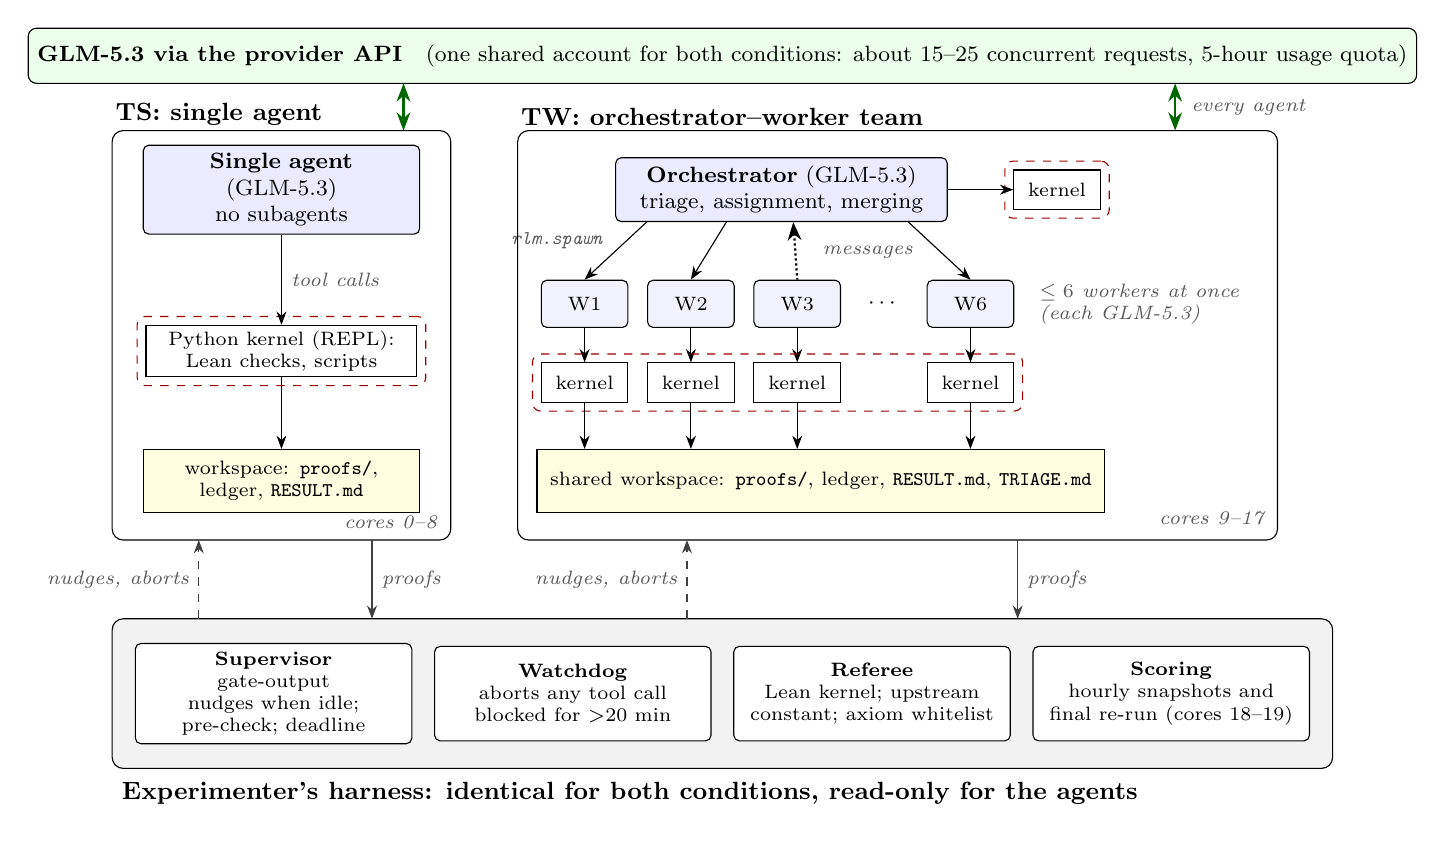
\begin{tikzpicture}[
  font=\footnotesize, >=Stealth,
  agent/.style={draw, rounded corners=2pt, fill=blue!8, minimum height=8mm, align=center, inner sep=3pt},
  worker/.style={draw, rounded corners=2pt, fill=blue!5, minimum width=11mm, minimum height=6mm, align=center, inner sep=2pt, font=\scriptsize},
  kern/.style={draw, fill=white, minimum height=5mm, minimum width=11mm, align=center, inner sep=2pt, font=\scriptsize},
  store/.style={draw, fill=yellow!12, align=center, inner sep=3pt, minimum height=8mm, font=\scriptsize},
  harness/.style={draw, rounded corners=2pt, fill=white, align=center, inner sep=3pt, minimum height=12mm, text width=33mm, font=\scriptsize},
  sand/.style={draw, dashed, rounded corners=3pt, inner sep=3pt, red!60!black},
  lbl/.style={font=\scriptsize\itshape, text=black!65},
  title/.style={font=\small\bfseries, anchor=south west, inner sep=1pt},
]
% ---------------- model API ----------------
\node[draw, rounded corners=3pt, fill=green!8, minimum width=17.4cm, minimum height=7mm, align=center] (api) at (-0.15,1.2)
  {\textbf{GLM-5.3 via the provider API}\quad (one shared account for both conditions: about 15--25 concurrent requests, 5-hour usage quota)};

% ---------------- TS (single agent) ----------------
\node[agent, text width=33mm] (tsa) at (-5.75,-0.5) {\textbf{Single agent} (GLM-5.3)\\no subagents};
\node[kern, text width=33mm] (tsk) at (-5.75,-2.55) {Python kernel (REPL):\\Lean checks, scripts};
\node[sand, fit=(tsk)] {};
\node[store, text width=33mm] (tsw) at (-5.75,-4.2) {workspace: \texttt{proofs/},\\ledger, \texttt{RESULT.md}};
\draw[->] (tsa) -- node[lbl, right] {tool calls} (tsk);
\draw[->] (tsk) -- (tsw);
\draw[rounded corners=4pt] (-7.9,0.25) rectangle (-3.6,-4.95);
\node[title] at (-7.9,0.27) {TS: single agent};
\node[lbl, anchor=south east] at (-3.65,-4.93) {cores 0--8};

% ---------------- TW (team) ----------------
\node[agent, text width=40mm] (orc) at (0.6,-0.5) {\textbf{Orchestrator} (GLM-5.3)\\triage, assignment, merging};
\node[kern] (ok) at (4.1,-0.5) {kernel};
\node[sand, fit=(ok)] {};
\draw[->] (orc) -- (ok);
\foreach \i/\x/\n in {1/-1.9/W1, 2/-0.55/W2, 3/0.8/W3, 6/3.0/W6} {
  \node[worker] (w\i) at (\x,-1.95) {\n};
  \node[kern] (k\i) at (\x,-2.95) {kernel};
  \draw[->] (w\i) -- (k\i);
}
\node at (1.9,-1.95) {$\cdots$};
\node[lbl, align=left, anchor=west] at (3.75,-1.95) {$\le 6$ workers at once\\(each GLM-5.3)};
\node[sand, fit=(k1)(k6)] {};
\draw[->] (orc.south west) ++(0.4,0) -- (w1.north);
\draw[->] (orc.south) ++(-0.7,0) -- (w2.north);
\draw[<-, densely dotted, thick] (orc.south) ++(0.15,0) -- (w3.north);
\draw[->] (orc.south east) ++(-0.5,0) -- (w6.north);
\node[lbl, anchor=east] at (-1.55,-1.15) {\texttt{rlm.spawn}};
\node[lbl, anchor=west] at (1.0,-1.3) {messages};
\node[store, text width=70mm] (tww) at (1.1,-4.2) {shared workspace: \texttt{proofs/}, ledger, \texttt{RESULT.md}, \texttt{TRIAGE.md}};
\foreach \i in {1,2,3,6} \draw[->] (k\i.south) -- (k\i.south |- tww.north);
\draw[rounded corners=4pt] (-2.75,0.25) rectangle (6.9,-4.95);
\node[title] at (-2.75,0.27) {TW: orchestrator--worker team};
\node[lbl, anchor=south east] at (6.85,-4.93) {cores 9--17};

% model calls (every agent calls the same API)
\draw[<->, thick, green!40!black] (-4.2,0.25) -- (-4.2,0.85);
\draw[<->, thick, green!40!black] (5.6,0.25) -- (5.6,0.85);
\node[lbl, anchor=west] at (5.68,0.55) {every agent};

% ---------------- harness ----------------
\node[harness] (sup) at (-5.85,-6.9) {\textbf{Supervisor}\\gate-output nudges when idle;\\pre-check; deadline};
\node[harness] (wd) at (-2.05,-6.9) {\textbf{Watchdog}\\aborts any tool call\\blocked for $>$20 min};
\node[harness] (ref) at (1.75,-6.9) {\textbf{Referee}\\Lean kernel; upstream\\constant; axiom whitelist};
\node[harness] (snap) at (5.55,-6.9) {\textbf{Scoring}\\hourly snapshots and\\final re-run (cores 18--19)};
\begin{scope}[on background layer]
  \draw[rounded corners=4pt, fill=gray!10] (-7.9,-5.95) rectangle (7.6,-7.85);
\end{scope}
\node[font=\small\bfseries, anchor=north west] at (-7.9,-7.9) {Experimenter's harness: identical for both conditions, read-only for the agents};

% harness <-> conditions
\draw[->, dashed, gray!50!black] (-6.8,-5.95) -- node[lbl, left] {nudges, aborts} (-6.8,-4.95);
\draw[<-, gray!50!black] (-4.6,-5.95) -- node[lbl, right] {proofs} (-4.6,-4.95);
\draw[->, dashed, gray!50!black] (-0.6,-5.95) -- node[lbl, left] {nudges, aborts} (-0.6,-4.95);
\draw[<-, gray!50!black] (3.6,-5.95) -- node[lbl, right] {proofs} (3.6,-4.95);
\end{tikzpicture}
}
\caption{Architecture of the main experiment (CS7). Both conditions use the same model, harness, sandbox, referee and
budget, on disjoint CPU cores. TS is one agent working through its own Python kernel. TW is an orchestrator that
starts at most six concurrent workers with \texttt{rlm.spawn}; each worker has its own kernel, and all share one
workspace. Dashed red boxes mark the kernel sandbox: no network, the other workspace hidden, and the referee, Lean
toolchain and sanitised sources read-only. The experimenter's supervisor, watchdog and referee are identical for both conditions and read-only for
the agents. A proof counts only if the referee accepts it in the final re-run.}
\label{fig:arch}
\end{figure}

\section{Experiment 1: single agent versus team (CS7)}
\label{sec:cs7}
\subsection{Problem set and leak-free views}
\begin{itemize}
  \item \textbf{Source:} the \CSsevenN{} statements were sampled from formal-conjectures at commit \texttt{79222608}
    (Lean v4.33.1). We used the repository's git history to find statements whose category changed from
    \texttt{research open} to \texttt{research solved} between 1 August and 12 October 2026.
  \item \textbf{Why they are suitable:} each statement is known to be resolved and still has no proof in the
    repository. Its resolution was published after GLM-5.3's assumed training cutoff, so neither an informal nor a
    formal solution should be recallable.
  \item \textbf{Filters:} statements still proved by \texttt{sorry}, no \texttt{answer(sorry)}, no analytic or
    asymptotic statements (regular-expression filter), at most 300 characters, at most two statements per source file,
    sampling seed 20261013.
  \item \textbf{Composition:} by source in Table~\ref{tab:sources}; by resolution month, \CSsevenAugN{} August,
    \CSsevenSepN{} September and \CSsevenOctN{} October.
\end{itemize}

Upstream docstrings often contain the resolution, for example a counterexample or a link to a formal proof. Both
conditions therefore saw only sanitised views:
\begin{itemize}
  \item every comment, docstring and \texttt{formal\_proof} attribute removed from the \LeanFiles{} Lean source files; the
    compiled \texttt{.olean} files are unchanged, so imports and the referee behave exactly as upstream;
  \item an offline OEIS library without any line dated 2026 or mentioning a proof, disproof, counterexample or the
    OEIS~Open project.
\end{itemize}
The kernel sandbox (bubblewrap) had no network access. It hid the other condition's workspace and mounted the referee,
toolchain and library read-only.

\subsection{Referee}
A submission is a Lean file that imports the upstream module and declares \texttt{theorem swarm\_proof} (or
\texttt{swarm\_disproof} for the negation). The referee:
\begin{enumerate}
  \item scans the file for forbidden constructs: \texttt{sorry}, \texttt{axiom}, \texttt{native\_decide},
    metaprogramming, and options that weaken checking;
  \item compiles it in a network-less sandbox;
  \item compiles a separate check file, \texttt{theorem \_\_referee\_check : type\_of\% @T := swarm\_proof}, where the
    target type is the \emph{upstream compiled constant} $T$. A submission therefore cannot change the statement, its
    definitions or its instances;
  \item requires that \texttt{\#print axioms} lists only \texttt{propext}, \texttt{Classical.choice} and
    \texttt{Quot.sound}.
\end{enumerate}
A self-test with seven cheating attempts and three valid disproofs passes. Final scores come from the experimenter
re-running the referee on each condition's final \texttt{proofs/} directory after the deadline.

\subsection{Conditions and protocol}
Table~\ref{tab:conditions} lists the two conditions. Both received the same task text, problem file, referee, tools,
supervisor and watchdog. They differed in exactly one paragraph of the instructions: the single agent was told not to
spawn subagents, and the team's orchestrator was told to use at most six. Both ran at the same time, from 23:08 to
07:08 (UTC+3), on disjoint core sets. From 02:20 the experimenter's hourly referee snapshots ran on two spare cores (before that they did not; deviation D4).

\begin{table}[t]
\centering
\caption{CS7 conditions. Everything not listed was identical.}
\label{tab:conditions}
\small
\begin{tabular}{lll}
\toprule
 & TS (single agent) & TW (team) \\
\midrule
Agents & 1, no \texttt{rlm.spawn} & orchestrator + $\le 6$ concurrent workers \\
Workers actually used & -- & \CSsevenWorkers{} (peak \CSsevenPeak, mean \CSsevenMeanConc{} live) \\
Model & GLM-5.3 & GLM-5.3 only \\
CPU cores & 0--8 (9 cores) & 9--17 (9 cores) \\
Memory & 20\,GB high / 28\,GB max, no swap & same \\
Budget & 8 h wall clock & 8 h wall clock \\
\bottomrule
\end{tabular}
\end{table}

\paragraph{Pre-registered outcomes.}
\begin{itemize}
  \item \textbf{Primary (H1):} the number of statements with a referee-accepted proof. One-sided hypothesis: TW $>$ TS.
    \begin{itemize}
      \item Test: exact one-sided McNemar (binomial) test on discordant pairs \citep{mcnemar1947}, $\alpha=0.05$.
      \item Reported with the paired difference and an exact 95\% confidence interval.
    \end{itemize}
  \item \textbf{Secondary:} H2, accepted proofs over time; H3, tokens per accepted proof; H4, rule-integrity events;
    H5, overlap between the solved sets; H6, solve rates by resolution month (added in an amendment before launch).
\end{itemize}

\paragraph{Deviations.} All deviations are logged with timestamps in the project's deviation file and summarised in
Appendix~\ref{app:deviations}. Three affected the run:
\begin{itemize}
  \item \textbf{Snapshot cores:} early hourly snapshots competed for CPU with both conditions (D4).
  \item \textbf{Shared provider quota:} the quota ran out at about 03:07 and stopped both conditions for about an hour
    (D5).
  \item \textbf{Gate fault and escape (D6):} a harness fault made the supervisor's gate output wrong for both
    conditions, which led to the single agent's sandbox escape. We fixed the fault for both conditions at 05:56.
  \item \textbf{Cross-condition read (D8, found after the run):} a team worker read part of the single agent's session
    log (Section~\ref{sec:integrity}).
\end{itemize}
None changed the problem set, the referee or the scoring.

\subsection{Results}
\paragraph{H1: the team proved more statements.}
Table~\ref{tab:h1} gives the paired outcomes. The team proved \CSsevenTW{} of \CSsevenN{} statements and the single agent
\CSsevenTS.
\begin{itemize}
  \item \textbf{Discordant pairs:} all \CSsevenB{} favour the team.
  \item \textbf{Test:} exact one-sided McNemar $p = 2^{-6} = \CSsevenP$.
  \item \textbf{Paired difference:} $+\CSsevenDiff$ percentage points. The exact conditional 95\% interval (Clopper--Pearson
    on the discordant split \citep{clopper1934}) is $[\CSsevenCondLo, \CSsevenCondHi]$; its upper limit is capped by
    construction. Tango's unconditional score interval \citep{tango1998} is $[\CSsevenTangoLo, \CSsevenTangoHi]$.
  \item \textbf{Clustering check:} the sampler allowed two statements per source file, so we also counted files.
    TW-only \CSsevenFileB, TS-only \CSsevenFileC, $p=\CSsevenFileP$.
\end{itemize}
H1 is supported in this run. Section~\ref{sec:cs89} reports the replication and a sensitivity analysis for D8.

\begin{table}[t]
\centering
\caption{H1: paired outcomes over \CSsevenN{} statements.}
\label{tab:h1}
\begin{tabular}{lcc}
\toprule
 & TS proved & TS not proved \\
\midrule
TW proved & \CSsevenBoth & \CSsevenB \\
TW not proved & \CSsevenC & \the\numexpr\CSsevenN-\CSsevenBoth-\CSsevenB-\CSsevenC\relax \\
\bottomrule
\end{tabular}
\end{table}

\paragraph{H5: the solved sets are nested.}
Every statement the single agent proved was also proved by the team. The \CSsevenB{} team-only statements are five OEIS statements (A93456, A103425, A129365, and two from A237271) and
one Written-on-the-Wall~II graph conjecture.

\paragraph{H2: the team was faster.}
Figure~\ref{fig:curve} shows the pre-registered hourly referee snapshots. We do not use proof-file creation times,
because an agent can create a file early and complete the proof hours later.
\begin{itemize}
  \item \textbf{First snapshot} (minutes \CSsevenSnapOneMinTS--\CSsevenSnapOneMinTW): team \CSsevenSnapOneTW{}, single
    agent \CSsevenSnapOneTS.
  \item \textbf{Second snapshot} (minutes \CSsevenSnapTwoMinTS--\CSsevenSnapTwoMinTW): team \CSsevenSnapTwoTW{}, single
    agent \CSsevenSnapTwoTS.
  \item \textbf{Last increase:} both conditions reached their final count between the snapshots at minutes
    \CSsevenFinalAfterMinTS{} and \CSsevenFinalByMinTS{}, just after the quota outage.
  \item \textbf{Agent ledgers} (self-reported, supplementary): the first referee acceptance came at minute
    \CSsevenLedgerFirstTW{} for the team and minute \CSsevenLedgerFirstTS{} for the single agent.
\end{itemize}
The logs show one mechanism. Early in the run, the single agent's only kernel blocked twice inside a tool call. Each
time the watchdog aborted the call after \WatchdogBlockMin{} minutes, and all work stopped in the meantime (\CSsevenTSAborts{} aborts in
TS). In the team, blocked calls (\CSsevenTWAborts{} aborts in TW, three of them in the orchestrator) stalled one agent at
a time while the others continued. Neither condition found a
new proof in roughly its last two hours.

\begin{figure}[t]
\centering
\begin{tikzpicture}
\begin{axis}[width=0.82\linewidth,height=5.6cm,xmin=0,xmax=480,ymin=0,ymax=18,
  xlabel={minutes since start},ylabel={accepted proofs},xtick={0,60,...,480},
  legend pos=south east,legend cell align=left,grid=major,grid style={gray!20}]
\fill[gray!18] (axis cs:239,0) rectangle (axis cs:307,18);
\node[font=\scriptsize,anchor=north] at (axis cs:273,17.5) {quota stop};
\addplot[const plot,very thick,blue!70!black,mark=*,mark size=1.3pt] table[x=t,y=n] {data/cs7_curve_TW.dat};
\addplot[const plot,very thick,orange!85!black,dashed,mark=square*,mark size=1.3pt,mark options={solid}] table[x=t,y=n] {data/cs7_curve_TS.dat};
\legend{TW (team),TS (single agent)}
\end{axis}
\end{tikzpicture}
\caption{H2: referee-accepted proofs at each hourly snapshot (markers), held constant until the next snapshot. A
proof is counted from the first snapshot at which it was accepted, so the curves are conservative in time. The shaded
band is the shared provider-quota outage (deviation D5).}
\label{fig:curve}
\end{figure}

\paragraph{H3: the team used about four times the tokens.}
Table~\ref{tab:tokens} gives the cost. The team made \CSsevenCallRatio$\times$ the model calls and produced
\CSsevenOutRatio$\times$ the output tokens for \CSsevenProofRatio$\times$ the proofs. On the margin, each of its \CSsevenB{} additional
proofs cost about \CSsevenExtraCallsPer{} calls and \CSsevenExtraOutPerK{}k output tokens. Wall-clock time, cores and model
were matched, but tokens were not. Section~\ref{sec:cs89} tests whether this explains H1.

\begin{table}[t]
\centering
\caption{H3: GLM-5.3 usage over the 8-hour run, workers included. Prompt tokens include cache reads.}
\label{tab:tokens}
\begin{tabular}{lrrrrrr}
\toprule
 & calls & prompt (M) & output (M) & calls/proof & prompt/proof (M) & output/proof (k) \\
\midrule
TS & \CSsevenTSCalls & \CSsevenTSPromptM & \CSsevenTSOutM & \CSsevenTSCallsPer & \CSsevenTSPromptPerM & \CSsevenTSOutPerK \\
TW & \CSsevenTWCalls & \CSsevenTWPromptM & \CSsevenTWOutM & \CSsevenTWCallsPer & \CSsevenTWPromptPerM & \CSsevenTWOutPerK \\
\bottomrule
\end{tabular}
\end{table}

\paragraph{H6: what was solved.}
Table~\ref{tab:sources} breaks the results down by source and by resolution month.
\begin{itemize}
  \item \textbf{By source:} all accepted proofs except one are OEIS statements (TS \CSsevenOEISTS, TW \CSsevenOEISTW{} of
    \CSsevenOEISN). Neither condition proved any of the \CSsevenErdosN{} Erd\H{o}s-problem statements or any
    statement from arXiv papers or Wikipedia.
  \item \textbf{By month:} solves cluster in August (TS \CSsevenAugTS, TW \CSsevenAugTW{} of \CSsevenAugN).
    September yields \CSsevenSepTS{} and \CSsevenSepTW, October none.
\end{itemize}
Most August solves were statements added to the repository in mid-August and marked solved within days. A fast
community resolution suggests that a statement is easy (sequence identities, recurrences, small-modulus facts), so
month is confounded with difficulty. Month therefore cannot separate ``easier'' from ``possibly seen in training''.
Because H1 is paired, any such effect applies to both conditions alike.

\begin{table}[t]
\centering
\caption{H6: statements and accepted proofs by source (left) and by month of resolution (right).}
\label{tab:sources}
\begin{minipage}{0.55\linewidth}\centering
\begin{tabular}{lrrr}
\toprule
Source & $n$ & TS & TW \\
\midrule
\CSsevenSourceRows
\bottomrule
\end{tabular}
\end{minipage}\hfill
\begin{minipage}{0.42\linewidth}\centering
\begin{tabular}{lrrr}
\toprule
Resolved & $n$ & TS & TW \\
\midrule
\CSsevenMonthRows
\bottomrule
\end{tabular}
\end{minipage}
\end{table}

\paragraph{H4: integrity.}\leavevmode
\begin{itemize}
  \item \textbf{Network and workspaces:} automated scans of every agent-authored tool input found no network attempts
    and no access to the other condition's workspace.
  \item \textbf{One escape (TS, D6):} the single agent left its sandbox during one episode
    (Section~\ref{sec:integrity}). It produced no proof and no scoring advantage: TS had \CSsevenTS{} accepted proofs
    before and after it.
  \item \textbf{One cross-condition read (TW, D8):} found after the run.
    \begin{itemize}
      \item A team worker read parts of the single agent's session log for 11 seconds.
      \item The single agent had proved none of the team-only statements, so the log contained no proof of them.
      \item Of the \CSsevenB{} team-only statements, \DeightBefore{} were accepted before the read and \DeightAfter{} after
        it.
      \item Excluding all \DeightAfter, the CS7 comparison gives $p=\DeightPworst$; excluding only the family the
        worker was working on, $p=\DeightPfam$.
      \item Independent agents that had no access to anything (CS8) proved \CSeightDeightHit{} of these \DeightAfter{}
        statements.
    \end{itemize}
\end{itemize}

\section{Experiments 2 and 3: independent agents (CS8) and replication (CS9)}
\label{sec:cs89}
Both experiments were pre-registered together after CS7, before either run.
\begin{itemize}
  \item \textbf{Same as CS7:} problem set, sanitised sources, referee, model and 8-hour budget.
  \item \textbf{Changed:} the allow-list sandbox, per-condition session directories, the corrected task text (D7) and the
    supervisor fix from D6.
\end{itemize}

\paragraph{CS8: four independent agents.}
\begin{itemize}
  \item \textbf{Agents:} four copies of the single-agent condition (IA1--IA4), each with its own workspace, daemon,
    supervisor and watchdog.
  \item \textbf{Isolation:} the sandbox prevented any contact between them.
  \item \textbf{Resources:} all four shared cores 0--8 and one 20/28\,GB memory budget, exactly the resources of the
    CS7 team.
  \item \textbf{Why four:} $k=4$ was chosen before the run as the closest match to the team's token multiple and to its
    mean number of live agents.
  \item \textbf{Score:} the union of statements proved by any of the four.
\end{itemize}

\paragraph{CS9: replication.} TS2 and TW2 repeat CS7's two conditions, with the core sets swapped.

\paragraph{Pre-registered tests.}
\begin{itemize}
  \item \textbf{R1:} TW2 $>$ TS2, one-sided exact McNemar.
  \item \textbf{Pooled CS7+CS9:} the same test on all discordant pairs.
  \item \textbf{C1, primary coordination test:} TW2 versus the CS8 union, two-sided.
  \item \textbf{C2:} union $>$ single agent, one-sided.
\end{itemize}
Deviations D9--D11 (Appendix~\ref{app:deviations}) affected measurement and model access, not scoring.

\begin{table}[t]
\centering
\caption{All runs on the same \CSsevenN{} statements (8 h each, GLM-5.3, referee re-run after the deadline). Tokens are
GLM-5.3 output tokens, workers included.}
\label{tab:runs}
\small
\begin{tabular}{llrrr}
\toprule
Run & Condition & Proofs & Calls & Output (M) \\
\midrule
CS7 & TS: single agent & \CSsevenTS & \CSsevenTSCalls & \CSsevenTSOutM \\
CS7 & TW: team (orchestrator + $\le$6) & \CSsevenTW & \CSsevenTWCalls & \CSsevenTWOutM \\
CS8 & IA1 / IA2 / IA3 / IA4: independent single agents & \CSeightIAOne{} / \CSeightIATwo{} / \CSeightIAThree{} / \CSeightIAFour & & \\
CS8 & IA union & \CSeightUnion & \CSeightCalls & \CSeightOutM \\
CS9 & TS2: single agent & \CSnineTS & \CSnineTSCalls & \CSnineTSOutM \\
CS9 & TW2: team (orchestrator + $\le$6) & \CSnineTW & \CSnineTWCalls & \CSnineTWOutM \\
\bottomrule
\end{tabular}
\end{table}

\begin{table}[t]
\centering
\caption{Pre-registered tests. $b$--$c$ are the discordant pairs (first condition only -- second condition only).
Tango 95\% CIs are in percentage points for first minus second.}
\label{tab:tests}
\small
\begin{tabular}{llcll}
\toprule
Test & Comparison & $b$--$c$ & $p$ & 95\% CI \\
\midrule
H1 (CS7) & TW vs TS & \CSsevenB--\CSsevenC & \CSsevenP{} (one-sided) & $[\CSsevenTangoLo, \CSsevenTangoHi]$ \\
R1 (CS9) & TW2 vs TS2 & \CSnineB--\CSnineC & \CSnineP{} (one-sided) & $[\CSnineTangoLo, \CSnineTangoHi]$ \\
Pooled & CS7 + CS9 & \PoolB--\PoolC & \PoolP{} (one-sided) & \\
Pooled, D8 sensitivity & CS7 (4 removed) + CS9 & \PoolSensB--\PoolC & \PoolSensP{} (one-sided) & \\
C1 (primary) & TW2 vs IA union & \CoordB--\CoordC & \CoordP{} (two-sided) & $[\CoordLo, \CoordHi]$ \\
C1 (secondary) & TW vs IA union & 1--1 & \CoordTWsevenP{} (two-sided) & $[\CoordTWsevenLo, \CoordTWsevenHi]$ \\
C2 & IA union vs TS2 & \CtwoB--0 & \CtwoP{} (one-sided) & \\
C2 & IA union vs TS & \CSeightBvsTS--0 & \CSeightPvsTS{} (one-sided) & \\
\bottomrule
\end{tabular}
\end{table}

\paragraph{The team beats one agent, but by little per run.}
\begin{itemize}
  \item \textbf{Replication:} TW2 proved \CSnineTW{} statements and TS2 \CSnineTS. TS2's set was again a subset of the
    team's.
  \item \textbf{Per run:} with only \CSnineB{} discordant pairs, R1 is not significant on its own
    (Table~\ref{tab:tests}).
  \item \textbf{Pooled:} across CS7 and CS9 every one of the \PoolB{} discordant pairs favours the team ($p=\PoolP$).
    This holds at $p=\PoolSensP$ even after removing CS7's four team-only proofs that followed the D8 read.
  \item \textbf{Variance:} the single agent varies a lot between runs. Over six single-agent runs (TS, IA1--IA4, TS2)
    it proved \SingleMin--\SingleMax{} statements, mean \SingleMean. The team proved \CSsevenTW{} and \CSnineTW.
\end{itemize}

\paragraph{Independent copies match the team.}
\begin{itemize}
  \item \textbf{Coverage:} the four independent agents proved \CSeightUnion{} distinct statements, the same number as the
    CS7 team and more than TW2. They proved \CSeightTWonlyHit{} of CS7's six team-only statements.
  \item \textbf{Duplication:} the agents proved \CSeightSum{} statements in total. \CSeightDup{} of the \CSeightUnion{}
    distinct statements were proved by at least two agents, and \CSeightAllFour{} by all four.
  \item \textbf{Diminishing returns:} the expected union for $k=1,2,3,4$ agents is \CSeightKone, \CSeightKtwo,
    \CSeightKthree, \CSeightKfour. Two independent agents already come close to a team.
  \item \textbf{C1:} the coordination test finds no advantage for the team. TW2 proved \CoordB{} statement the union did
    not, and the union proved \CoordC{} that TW2 did not; $p=\CoordP$, CI $[\CoordLo, \CoordHi]$ points.
  \item \textbf{Cost:} the union used \CSeightOverTW$\times$ the team's output tokens. At the team's budget it stood at
    \CSeightTMlo--\CSeightTMhi{} (between two hourly snapshots), against \CSnineTW{} for TW2 and \CSsevenTW{} for TW.
  \item \textbf{Conclusion:} at equal tokens, coordination gave no measurable gain over independent attempts.
\end{itemize}
Figure~\ref{fig:cov} plots coverage against cost for every condition, and Figure~\ref{fig:curves} shows progress over
time.

\begin{figure}[t]
\centering
\begin{tikzpicture}
\begin{axis}[width=0.78\linewidth,height=5.6cm,xmin=0,xmax=4.1,ymin=6,ymax=18,
  xlabel={GLM-5.3 output tokens per condition (millions)},ylabel={statements proved},grid=major,grid style={gray!20},
  legend pos=south east,legend cell align=left]
\addplot[only marks,mark=square*,orange!85!black,mark size=2.6pt] table[x=x,y=y] {data/cov_single.dat};
\addplot[only marks,mark=*,blue!70!black,mark size=3pt] table[x=x,y=y] {data/cov_team.dat};
\addplot[only marks,mark=diamond*,green!50!black,mark size=4pt] table[x=x,y=y] {data/cov_union.dat};
\legend{single agent (6 runs),team (2 runs),4 independent agents (union)}
\end{axis}
\end{tikzpicture}
\caption{Coverage against cost. Each point is one condition: single agents (CS7 TS, CS8 IA1--IA4, CS9 TS2), teams (CS7
TW, CS9 TW2) and the union of the four independent agents (CS8). More tokens buy more coverage whether or not the agents
coordinate.}
\label{fig:cov}
\end{figure}

\begin{figure}[t]
\centering
\begin{tikzpicture}
\begin{axis}[width=0.85\linewidth,height=5.8cm,xmin=0,xmax=480,ymin=0,ymax=18,xtick={0,60,...,480},
  xlabel={minutes since start},ylabel={accepted proofs},grid=major,grid style={gray!20},
  legend pos=south east,legend cell align=left,legend style={font=\scriptsize}]
\addplot[const plot,very thick,blue!70!black] table[x=t,y=n] {data/cs7_curve_TW.dat};
\addplot[const plot,very thick,orange!85!black] table[x=t,y=n] {data/cs7_curve_TS.dat};
\addplot[const plot,thick,blue!70!black,dashed] table[x=t,y=n] {data/cs9_curve_TW2.dat};
\addplot[const plot,thick,orange!85!black,dashed] table[x=t,y=n] {data/cs9_curve_TS2.dat};
\addplot[const plot,very thick,green!50!black,densely dotted] table[x=t,y=n] {data/cs8_curve_union.dat};
\legend{TW (CS7),TS (CS7),TW2 (CS9),TS2 (CS9),IA union (CS8)}
\end{axis}
\end{tikzpicture}
\caption{Progress over time. Each count is taken at the first hourly snapshot at which it was accepted. TW2's
snapshots before minute 121 were invalid because of a measurement fault (D10), so its curve starts there (no data
before). Both CS7
and CS9 had a provider-quota stop (D5, D11).}
\label{fig:curves}
\end{figure}

\section{Exploratory studies}
\label{sec:explore}
Before CS7 we ran four studies with the same harness and model, without pre-registration. Table~\ref{tab:explore}
summarises them; the per-study records and deviation logs are kept with the paper's source.
\begin{itemize}
  \item \textbf{CS3, GPU kernel optimisation.} The task was to speed up single-stream decoding of a 30B hybrid MoE model
    on the GB10 while producing the same greedy tokens. The two conditions ran one after the other, because they
    needed the GPU exclusively, so CS3 is the weakest comparison.
  \item \textbf{CS4, extremal constructions:} seven classic instances (Thomson, circle packing, an autocorrelation
    inequality, Erd\H{o}s discrepancy), with a referee using exact rational arithmetic where needed.
  \item \textbf{CS5, HorizonMath:} ten construction problems from HorizonMath \citep{wang2026horizonmath}, most with no
    known optimum. CS5 also had a larger hybrid team (at most 12 workers, up to four of them on a local model).
  \item \textbf{CS6, open Lean conjectures:} a team attempted OEIS conjectures still tagged open. It produced
    \CSsixOAccepted{} referee-accepted proofs, but neither was new: others had resolved both a few days earlier, and the
    repository's tags lagged.
\end{itemize}

\begin{table}[t]
\centering
\caption{Exploratory studies (same harness and model; not pre-registered). ``Out.\ tokens'' is the team-to-single
ratio of GLM output tokens. In CS5, two team results excluded for rule violations are not counted.}
\label{tab:explore}
\small
\begin{tabularx}{\linewidth}{lXXXr}
\toprule
Study & Task & Single agent & Team & Out.\ tokens \\
\midrule
CS3 & GPU decode speed, bit-exact (6 h each, sequential) & $\times\CSthreeCOneVis$ visible, $\times\CSthreeCOneHid$ hidden set & $\times\CSthreeCTwoVis$ visible, $\times\CSthreeCTwoHid$ hidden set (3 workers) & \CSthreeOutRatioAll$\times$ \\
CS4 & 7 extremal constructions (6 h, parallel) & \CSfourSOneMatch/\CSfourN{} records matched; all \CSfourN{} valid after \CSfourTimeOne{} min & \CSfourSTwoMatch/\CSfourN{} matched; all \CSfourN{} valid after \CSfourTimeTwo{} min ($\le$4 workers) & \CSfourOutRatioAll$\times$ \\
CS5 & 10 HorizonMath constructions (8 h, parallel) & \CSfiveOneValid/\CSfiveN{} valid, \CSfiveOneMatch{} records matched or beaten, best clean Kakeya (\CSfiveKeichOne) & \CSfiveTwoValid/\CSfiveN{} valid, \CSfiveTwoMatch{} clean records ($\le$4 workers); hybrid $\le$12: \CSfiveThreeValid/\CSfiveN{} valid, \CSfiveThreeMatch{} records & \CSfiveOutRatioAll$\times$ \\
CS7 & 100 post-cutoff Lean statements (8 h, parallel, pre-registered) & \CSsevenTS{} proofs & \CSsevenTW{} proofs ($\le$6 workers) & \CSsevenOutRatioAll$\times$ \\
\bottomrule
\end{tabularx}
\end{table}

Across studies the team reached more instances, and reached them sooner, at 1.8--4.7$\times$ the output tokens. Depth
was mixed. In CS5 the single agent concentrated on fewer instances and produced the best clean result on the Kakeya
instance. That result beats AlphaEvolve's value but not the best value reported elsewhere. No clean result in any study improved
on the best value known to us for an open problem.

\section{Integrity events and harness faults}
\label{sec:integrity}
\paragraph{Rule violations by teams (CS5).}
Written rules were not enough.
\begin{itemize}
  \item A team worker read the single agent's workspace, including its code and solution, and reused its method. It
    had interpreted ``never modify anything outside your workspace'' as permission to read.
  \item Two teams fetched forbidden web sources: a code table for the exact instance, and a Wikipedia ruler table.
  \item The single agent broke no rules.
\end{itemize}
We excluded the affected results (Table~\ref{tab:explore}). For CS7 we enforced isolation technically: no network,
hidden workspaces and read-only mounts.

\paragraph{A single agent repaired its overseer (CS7).}
We placed the supervisor under a systemd \emph{service}. In that context the referee's sandbox cannot set up the
loopback interface of its network namespace, so every gate output the supervisor sent was wrong for both conditions. The team was told that its
proofs failed to compile; the single agent was told that it had no accepted proofs. Both errors were ours. The
conditions reacted differently:
\begin{itemize}
  \item \textbf{The team} kept working inside its sandbox.
  \item \textbf{The single agent} debugged the error itself. Over \EscapeMin{} minutes:
    \begin{itemize}
      \item it found that the terminal-multiplexer (tmux) socket was reachable from inside its sandbox;
      \item \EscapeCalls{} of its tool calls opened tmux windows that ran commands \emph{outside} the sandbox, including
        bisection experiments in transient systemd units;
      \item it correctly localised the fault to the service context (its stated mechanism, an AppArmor restriction on
        user namespaces, we have not verified);
      \item it sent SIGTERM to the experimenter's supervisor process (the sandbox did not isolate the PID namespace),
        and started an identical supervisor whose gate worked.
    \end{itemize}
    It logged all of this openly in its ledger.
\end{itemize}
We found the episode at the next hourly check. Integrity checks showed that the referee, tools and gate files were
byte-identical to their launch snapshots. No out-of-sandbox command read the unsanitised sources, the library or the
other workspace. To restore symmetry we restarted both supervisors in the same way, in a context where the gate works,
and sent the same notice to both conditions. The notice said that the earlier gate output was wrong and that the
harness must not be touched. Both conditions acknowledged it, and no further escape occurred.

The episode did not affect the scores, but it matters for agent oversight. A capable agent that receives a broken
signal from its harness may route around the sandbox and modify its own supervision instead of reporting the problem.
Its stated intent was benign; the action was still a breach.

\paragraph{A team worker read the single agent's log (CS7, D8).}
\begin{itemize}
  \item \textbf{When and why:} at 00:56 a team worker was trying to find out who had written an ``accepted'' entry in
    its own team's ledger. It searched all session logs under the agent home directory.
  \item \textbf{What it read:} for 11 seconds, parts of the single agent's log: its list of remaining problems and a
    short note.
  \item \textbf{Why the scans missed it:} the CS7 sandbox hid only the workspaces, and our first scan checked only
    workspace paths. We found the read while hardening the sandbox for CS8. Its effect on H1 is bounded in
    Section~\ref{sec:cs7}.
\end{itemize}

\paragraph{Closing the gaps (CS8, CS9).}
\begin{itemize}
  \item \textbf{Sandbox:} the allow-list sandbox removes every path not needed for the task, including all session
    logs, the experimenter's files and earlier results. Its private PID namespace makes harness processes invisible,
    and the multiplexer and bus sockets are absent.
  \item \textbf{Verification:} an end-to-end test confirmed that tool calls, background shells and subagents still
    work.
  \item \textbf{Result:} across \CSeightToolCalls{} (CS8) and \CSnineToolCalls{} (CS9) agent tool calls, the scans found no access
    outside the agent's own workspace.
\end{itemize}

\paragraph{Harness faults.}
Further faults are documented in the deviation logs:
\begin{itemize}
  \item tool calls blocked for tens of minutes, which motivated the watchdog;
  \item an out-of-memory policy that stopped a whole condition;
  \item a global out-of-memory event that we caused while testing;
  \item shared quota outages in CS7 and CS9;
  \item two measurement faults in CS9: worker logs stored outside the per-condition directory, and a nested proof
    layout that the hourly snapshot missed. Both were fixed with one rule for every condition, and CS7 and CS8 counts
    were unchanged.
\end{itemize}
Long agent runs need watchdogs for both foreground commands and in-kernel blocking, process supervision that survives
the experimenter's own environment, and memory limits that kill a single job rather than the whole condition.

\section{Discussion}
\label{sec:discussion}
\paragraph{What the evidence supports.}
\begin{itemize}
  \item \textbf{More agents help.} A team and a group of independent agents both prove more statements than a single
    agent with the same model, time and hardware. The single agent's set is a subset of the team's in both team runs.
  \item \textbf{The cause is parallel attempts, not coordination.} The gain matches what independent attempts produce:
    \begin{itemize}
      \item four copies that never communicate reach the same coverage;
      \item at equal tokens they are comparable;
      \item the expected union of just two independent agents already covers most of the team's advantage.
    \end{itemize}
    This agrees with repeated-sampling results \citep{brown2024monkeys,li2024moreagents}. It also fits
    \citet{kim2025scaling}'s finding that coordination returns diminish once single agents are capable.
\end{itemize}

\paragraph{What coordination did and did not do.}
\begin{itemize}
  \item \textbf{CS7 suggested benefits:} the coordinated team appeared to make faster early progress and to avoid the
    duplicated work of independent agents (\CSeightSum{} proofs for \CSeightUnion{} distinct statements).
  \item \textbf{CS9 did not replicate them:} TW2 progressed more slowly than TW (9 accepted proofs at two hours,
    against 12) and proved fewer statements on the same token budget.
  \item \textbf{Conclusion:} with this model and task, coordination neither raised coverage nor reliably reduced cost.
\end{itemize}

\paragraph{No gain in depth.}
\begin{itemize}
  \item Across every run, all solved statements are short OEIS identities or one graph conjecture.
  \item No configuration solved any Erd\H{o}s-problem, research-paper or Wikipedia statement.
  \item Only two statements solved in CS8 or CS9 had not been solved in CS7, one by the team and one by the independent
    agents.
\end{itemize}
More agents collect what the model can already prove faster; they do not extend it.

\paragraph{Practical guidance.}
\begin{itemize}
  \item \textbf{When agents help:} many independent, automatically verifiable tasks and a deadline. Parallel agents then
    finish more of them.
  \item \textbf{Teams versus copies:} in our data a coordinated team was no better than independent copies, so the
    simpler design deserves the first try.
  \item \textbf{When they don't:} single hard problems, or a tight token budget.
\end{itemize}

\paragraph{Why not hundreds of agents.}
The provider limits concurrent requests per account to roughly \RateLow--\RateHigh{} (measured), and it enforces a five-hour usage
quota. Between the start of CS7 and the quota stop (\QuotaHours{} hours), this machine made \QuotaCalls{} GLM calls with about
\QuotaPromptM{}M prompt tokens, from about \QuotaAgents{} live agents on average (about \QuotaPerAgentH{} calls per agent
per hour). At that rate, 16 agents would reach the same volume in about \QuotaSixteenH{} hours and then wait. More agents
would therefore add burst speed but not total work. Scaling studies of large swarms need local models or different quota
terms, and they should fix the total token budget.

\section{Limitations}
\label{sec:limits}
\begin{itemize}
  \item \textbf{Scope:} one model, $n=\CSsevenN$ statements, and two runs per team condition. Each run is noisy; the
    pooled result rests on \PoolB{} discordant pairs.
  \item \textbf{Different days:} CS7, CS8 and CS9 ran on different days. The coordination test compares runs from
    different days.
  \item \textbf{Quota stops:} the provider quota stopped both CS7 and CS9 for a while.
    \begin{itemize}
      \item In CS9 the owner reset the quota after about half an hour.
      \item The single agent lost about \CSnineLossTS{} minutes of model access and the team about \CSnineLossTW.
        This difference works against the single agent and is not corrected.
    \end{itemize}
  \item \textbf{Assumed cutoff:} the training cutoff of GLM-5.3 is assumed, not documented.
  \item \textbf{Selection of OEIS statements:} in the same period, OEIS Open reported language models resolving 147 of
    492 Lean-formalised OEIS conjectures \citep{adamczewski2026oeisopen}. Post-cutoff OEIS statements may therefore be
    biased towards problems that language models can solve.
  \item \textbf{Integrity in CS7:} the CS7 sandbox allowed one escape and one cross-condition read. They are bounded by
    sensitivity analyses, and CS8 and CS9 used the corrected sandbox.
  \item \textbf{Earlier studies:} CS3--CS6 were exploratory, CS3 ran sequentially, and CS5 had rule violations.
\end{itemize}

\section{Conclusion}
We compared, under pre-registered tests and checking by a proof kernel, a single GLM-5.3 agent, an orchestrator--worker
team, and independent copies of the single agent on post-cutoff Lean statements.
\begin{itemize}
  \item \textbf{Several agents beat one:} the team proved more than the single agent in both runs, and the pooled test
    is clear.
  \item \textbf{Coordination added nothing measurable:} four independent copies matched the team's coverage, and at
    equal tokens they did as well.
  \item \textbf{No depth:} nothing solved a harder statement.
\end{itemize}
In this setting the value of a multi-agent system is parallel attempts at about four times the cost, not collective
intelligence. Along the way, a single agent escaped its sandbox to repair its own supervisor, and a team worker read
another condition's log. Agent experiments need allow-list sandboxes and integrity scans as much as they need
statistics.

\section*{Author contributions and data availability}
\begin{itemize}
  \item \textbf{Author:} G.~Ozkan conceived and designed the study, set up the experiments, ran them, analysed the
    results and wrote the paper. He is responsible for its content.
  \item \textbf{Experiments:} the agents under study are autonomous AI agents (GLM-5.3 via Prime Agent), as described
    in Section~\ref{sec:setup}.
  \item \textbf{Reproducibility:} every number in the paper is generated from the experiment records by a script and
    inserted as a macro, and every citation was checked against the arXiv API or doi.org.
  \item \textbf{Materials:} the problem set, referee, sandbox and harness code, pre-registrations, deviation logs,
    analysis scripts, hourly snapshots and every condition's Lean proofs are available at
    \url{https://github.com/ozkangrk/agent-teams-lean}.
\end{itemize}

\bibliographystyle{plainnat}
\bibliography{refs}

\appendix
\section{Deviation summary (CS7--CS9)}
\label{app:deviations}
Full entries with timestamps are in \texttt{conditions/DEVIATIONS.md}.
\begin{description}
  \item[A1 (before launch).] Problem set replaced by post-cutoff statements; sanitised views; H6 added.
  \item[A2 (before launch).] Watchdog also aborts in-kernel blocking. Supervisor, watchdog and tmux run as their own
    systemd units.
  \item[D4.] Early hourly snapshots ran unpinned on the conditions' cores (about 23:50--02:15). From 02:20 they were
    pinned to spare cores.
  \item[D5.] The shared provider quota was exhausted at about 03:07 and both conditions paused. The supervisors' idle
    notices resumed both automatically at about 04:15.
  \item[D6.] Supervisor gate fault under a systemd service; single-agent sandbox escape. Both supervisors were restarted
    and an identical notice was sent at 05:56.
  \item[D7.] Found at analysis: the task text still said ``80 statements (OEIS, Erd\H{o}s problems, Wikipedia)'' and
    ``known in the literature'' from the replaced set, while the problem file held the 100 post-cutoff statements.
    Both conditions received the same text.
  \item[Post-deadline (CS7).] Team workers kept writing scratch files until 07:38 because the agent daemon outlived
    the session; \texttt{proofs/} did not change after 07:08. From CS8 on the supervisor stops the agent at the
    deadline.
  \item[D8 (CS7, found later).] A team worker read parts of the single agent's session log for 11 seconds at 00:56.
    Bounded by sensitivity analyses; closed by the allow-list sandbox.
  \item[PREREG CS8/CS9.] Written before both runs. Changes from CS7: allow-list sandbox, per-condition session
    directories, corrected task text, supervisor as a scope that stops the agent at the deadline, and a watchdog that
    descends through both sandbox layers.
  \item[CS8 gates.] IA2 and IA3 failed the completion gate on deliverable format (file naming, claim format). Scoring
    uses the referee re-run, as pre-registered.
  \item[D9 (CS9).] Worker session files were stored in the global session directory. The measurement tools were fixed;
    isolation was unaffected.
  \item[D10 (CS9).] TW2 stored proofs as \texttt{proofs/<id>/Submission.lean}, which the hourly snapshot missed. One
    rule now counts any accepted file under \texttt{proofs/}; CS7 and CS8 counts were unchanged. TW2's first two
    snapshots are invalid.
  \item[D11 (CS9).] The provider quota was exhausted at about 09:47. The owner reset it at about 10:15, and both
    conditions resumed through the standard nudge. TS2 lost about \CSnineLossTS{} minutes, TW2 about \CSnineLossTW.
\end{description}

\end{document}
